\documentclass[a4paper,12pt]{article}
%\DeclareMathSizes{display size}{text size}{script size}{scriptscript size}.

\title{\vspace{-1.7 cm} Notes on Assorted Project Euler Problems}
\author{Gavin S. Hartnett}

\usepackage{url}
\usepackage{amssymb}
\usepackage{amsmath}
\usepackage[left=1.8cm,right=1.8cm,top=2cm,bottom=2.0cm,nohead]{geometry}
\usepackage[usenames]{color}
\usepackage{epsfig,latexsym,amsfonts,amsmath,amsthm,amssymb,amsbsy,multirow,slashed,color,mathrsfs,wasysym,textcomp,subfigure,wrapfig,comment}
\usepackage{framed} 
\usepackage{parskip}
%\setlength{\parskip}{1cm plus4mm minus3mm}

\renewcommand{\rmdefault}{phv} %Arial
\renewcommand{\sfdefault}{phv} %Arial 
\newcommand{\BibTeX}{{\sc Bib}\TeX}
\newcommand{\blue}[1]{\textcolor{blue}{#1}}
\newcommand{\red}[1]{\textcolor{red}{#1}}

%\DeclareMathSizes{10000}{10000}{10000}{10000}

\date{}
\begin{document}
\maketitle
\vspace{-0.5cm}
%%%%%%%%%%%%%%%%%%%%%%%%%%%%%%%%%%%%%%%%%%%%%% Body %%%%%%%%%%%%%%%%%%%%%%%%%%%%%%%%%%%%%%%%%%%%%%
\section{Problem 140}
The first step is to sum the geometric series 
$$ A_G(x) = \sum_{k=1}^{\infty} x^k G_k \, . $$
To do so, we need a closed form expression for $G_k$. Such an expression exists for the Fibonacci numbers. I did some digging and found that for a recursion series of the form $G_k = G_{k-1} + G_{k-2}$, with $G_1 = a$, $G_2 = b$, the expression is
$$ G_k = \frac{1}{2} \left[ (3 a -b) F_k + (b-a) L_k \right] \, , $$
where $F_k, L_k$ are the $k$-th Fibonacci and Lucas numbers. In this particular case, 
$$ G_k = \left( \frac{15 - \sqrt{5}}{10} \right) y_-^k + \left( \frac{15 + \sqrt{5}}{10} \right) y_+^k \, , $$
where
$$ y_{\pm} \equiv \left( \frac{1 \pm \sqrt{5}}{2} \right)^k \, .$$
Summing up the geometric series gives
$$ A_G = \left( \frac{15 - \sqrt{5}}{10} \right) \frac{x y_-}{1- x y_-} + \left( \frac{15 + \sqrt{5}}{10} \right) \frac{x y_+}{1- x y_+} \, , $$
and we can solve for $x$ in terms of $A_G$:
$$ x = \frac{\sqrt{1+14 A_G + 5 A_G^2} - (A_G + 1)}{6 + 2 A_G} \, . $$
Now our task seems easy enough, in order for $x$ to be a ``Golden Nugget", we need $(1 + 14 A_G + 5 A_G^2)$ to be a perfect square so that $x$ is rational. The problem is that the perfect square values of $A_G$ become increasingly spread out. Below is a log plot of the first few:
\begin{figure}[h!]
\begin{center}
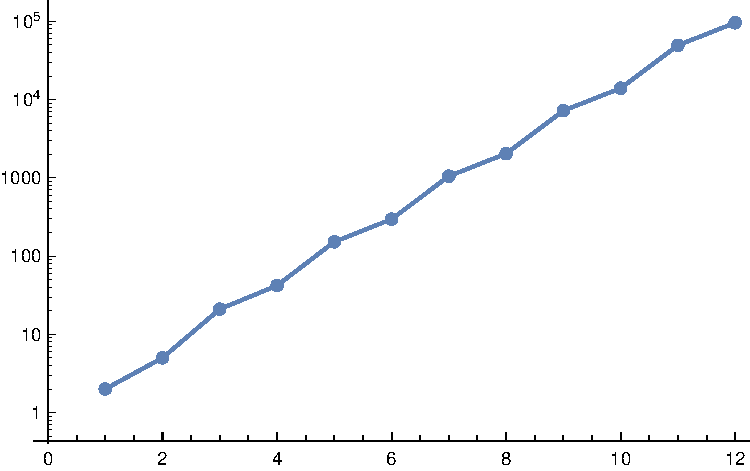
\includegraphics[width=0.5\textwidth]{Figures/p140.pdf}
\end{center}
\caption{The first few values of $A_G(x)$ for which $x$ is a Golden Nugget.}
%\label{fig:mincoupledscalarinstability}
\end{figure}

We'll need a more sophisticated method to find the solution since a simple scan will take an exponentially long time. It turns out that the question of when a polynomial such as 
$$ z^2 = 5 w^2 + 14 w + 1$$
has integer solutions (for both $w$ and $z$) is exactly what the Diophantine equations determine. I found that \textit{Mathematica} has a routine capable of solving these equations and implemented it, unfortunately learning very little in the process. I should revisit this.


%%%%%%%%%%%%%%%%%%%%%%%%%%
%Bibliography
%%%%%%%%%%%%%%%%%%%%%%%%%%
\bibliography{refs}{}
\bibliographystyle{utphys}

\end{document}